\documentclass{article}


% Font encoding and language
\usepackage[T1]{fontenc}
\usepackage[utf8]{inputenc}
\usepackage[english]{babel}

% For mathematical symbols and equations
\usepackage{amsmath, amssymb, amsfonts}

% For including graphics
\usepackage{graphicx}

% For customized section headings
\usepackage{titlesec}

% For setting margins
\usepackage[margin=1in]{geometry}
\usepackage{tikz}
\usetikzlibrary{arrows.meta, positioning, shapes.geometric}

\title{Math 585 Survey Paper : Ancient Murrlets, Multi-State and Multi-Event Models}
\author{Shay AhooeiNejad}
\date{Feb, 2024}


\begin{document}

\maketitle
\section{Abstract}

The Ancient Murrelet (Synthliboramphus antiquus), a charismatic seabird inhabiting the North Pacific, has captivated the attention of ornithologists and conservationists alike due to its intriguing behavior and ecological significance. Navigating the complex marine ecosystems, Ancient Murrelets are essential indicators of environmental health, reflecting the intricate balance between oceanic dynamics and avian populations. To gain deeper insights into their population dynamics and movement patterns, advanced analytical models are indispensable.

This study delves into the comprehensive analysis of Ancient Murrelet populations, employing three crucial models for enhanced understanding. The first model revolves around capture-recapture techniques, enabling the estimation of population size and survival rates. The second model, a multi-state approach, extends the analysis by incorporating distinct states within the bird's life cycle. Furthermore, recognizing the uncertainties inherent in ecological studies, the third model introduces the concept of "Multi-event," an extension of the multi-state model, adept at handling situations with incomplete or uncertain information. By employing these models, the research enhances our understanding of Ancient Murrelet ecology, paving the way for more nuanced conservation strategies in response to the dynamic challenges presented by their marine habitats.

\section{Ancient Murrelets:}

Ancient Murrelets (\textit{Synthliboramphus antiquus}), belonging to the family Alcidae, are small auks closely related to the Japanese Murrelet. This species comprises two races, one inhabiting the Commander Islands and the other near the Gulf of California, characterized by Craveri’s (\textit{S. craveri}) and Xantus’ (\textit{S. hypoleucus}) murrelets.\cite{bc_ancient_murrelet}

These small auks exhibit a distinctive appearance with a black bib, long white filamentous plumes along the crown's sides during breeding plumage, and a modest size with a 14 cm wing length, weighing between 200 to 250 g. Both males and females share similar physical characteristics, featuring a moderate grey back, upper wings, and upper tail, along with a black head, white belly, pale blue legs and feet, and a short, pointed, pinkish bill in adults.\cite{bc_ancient_murrelet}

The Ancient Murrelet's range forms an arc around the northern Pacific Ocean, encompassing breeding and feeding waters. In British Columbia, these birds primarily breed on offshore islands in the Queen Charlotte Islands/Haida Gwaii, with nesting colonies distributed across Graham and Moresby Islands. Notably, around 7\% of the population nests on small colonies off the northwest side of Moresby Island. During late summer and early fall, Ancient Murrelets are rarely sighted in British Columbia waters, as they migrate to winter in the marine waters around Vancouver Island.\cite{gaston1990population}

Their diet varies across regions and years, primarily consisting of large zooplankton and small schooling fish. Young-of-the-year Ancient Murrelets predominantly forage on sand lance, often forming small groups or mixed species feeding flocks.\cite{bc_ancient_murrelet}

Breeding in Ancient Murrelets is not strictly tied to latitude but is influenced by food supply rather than day length. They are colonial burrow-nesters, visiting colonies in March and laying eggs from 1 to 10 April. Incubation lasts about a month, and precocial chicks hatch within 12 hours of each other. Ancient Murrelets are confined to temperate and subarctic waters of the North Pacific, feeding in continental shelf waters, usually out of sight of land. Unlike other seabirds, Ancient Murrelet chicks are never fed at the colony. Instead, the two chicks leave at night, 2-4 days after hatching, travel out to sea, and are fed by their parents until fully grown, about 6-8 weeks old. The precocial behavior of young Ancient Murrelets, though unusual among seabirds, provides the species with the potential to rear a brood of two chicks. This departure strategy challenges the norm among seabirds, leading to speculation about its adaptive significance.\cite{bc_ancient_murrelet}\cite{gaston1990population}


While there is limited information on fidelity to natal colonies, some recruitment to non-natal colonies has been observed. Nest site fidelity is challenging to ascertain due to the birds nesting in burrows.\cite{gaston1990population}


Ancient Murrelets disperse from breeding colony waters once chicks join parents at sea, remaining in offshore waters for weeks before appearing at wintering grounds in late summer and early fall.

Nesting habitats consist of forested islands in the Queen Charlotte Islands/Haida Gwaii archipelago. The birds nest in burrows beneath mature Sitka spruce or western hemlock, predominantly on seaward slopes or flat areas.

The Canadian breeding population of Ancient Murrelets is around 256,000 pairs, with the B.C. population representing half of the global total. The presence of introduced mammalian predators on colony islands has rendered those islands unsuitable for nesting Ancient Murrelets. The main threats to the population include rats and raccoons, along with contaminants, ocean resource exploitation, human recreation, and the overarching impacts of climate change.\cite{gaston1990population}


Regarding their breeding status, adults' breeding status was determined by inspecting brood patches or finding birds with eggs or chicks, or was based on the date of capture. Retrapping of breeders estimated an annual survival rate of 77\%, which is lower than estimates for other alcids. Reproductive success under undisturbed conditions averaged 1.54 chicks per breeding pair per year, unusually high for an alcid. Nonbreeders visiting the colony were mainly in their second or third year, with breeding likely beginning in the third or fourth year. The high mortality of adult Ancient Murrelets on their breeding colonies could explain the evolution of their precocial departure strategy.\cite{gaston1990population}



\section{Capture-recapture}

Capture-recapture models are statistical tools employed in ecology and population biology to estimate the size of a population by capturing, marking, releasing, and subsequently recapturing individuals. The fundamental concept behind these models lies in the assumption that the proportion of marked individuals within a recaptured sample is representative of the total population.

The history of capture-recapture modeling dates back to the pioneering work of British statistician Sir Ronald A. Fisher in the early 20th century. Fisher's contributions laid the groundwork for population estimation methods, with his seminal paper "On the Mathematical Foundations of Theoretical Statistics" in 1922 being a cornerstone in statistical theory.

In the ecological context, the use of capture-recapture models gained momentum in the mid-20th century. The work of Leslie, Skalski, and Rykiel in the 1970s significantly contributed to the development and application of capture-recapture techniques in wildlife biology. Their efforts helped refine the models and expand their utility in estimating population sizes, survival rates, and other vital demographic parameters.

Notably, the Jolly-Seber model, introduced independently by Peter D. Jolly and Richard Ryding Seber in the early 1960s, has become a cornerstone in capture-recapture methodology. This model, along with subsequent extensions and variations, forms the basis for many contemporary population estimation studies.

Over the years, researchers like Cormack, Schwarz, and others have made substantial contributions to the refinement and application of capture-recapture models. Cormack's formulation of the Cormack-Jolly-Seber model further advanced the field, allowing for more sophisticated analyses of marked populations.

The evolution of capture-recapture models continues with modern advancements, integrating spatial and temporal components for a more comprehensive understanding of population dynamics. As researchers address new challenges in conservation biology and ecology, capture-recapture models remain invaluable tools for assessing and managing wildlife populations.


\section{Multi-State Models in Avian Ecology}

In avian ecology, understanding the survival dynamics of bird species, such as the Ancient Murrelet, has become more nuanced through advanced modeling techniques. This section delves into multi-state models, an extension of traditional capture-recapture approaches, to unravel the complexities of individual movement and survival.

Our study focuses on assessing the 'cost of reproduction' hypothesis, examining how increased breeding effort might influence the survival of bird species. The experimental design incorporates a control group alongside two treatment groups, 'addition' (increased offspring) and 'subtraction' (decreased offspring). Initial analysis, emphasizing return rates, revealed unexpected patterns, prompting a deeper examination of survival probability calculations.

\subsubsection*{Key Definitions} 


\textbf{Return Rates}

"Defined as the proportion of marked individuals encountered alive during subsequent sampling occasions, return rates provide insights into the survival dynamics of populations over specific time intervals".\cite{mark_website}

\textbf{Survival Probability}

"This probability represents the likelihood that a marked individual, having survived from one sampling occasion to the next, will be encountered alive in the subsequent period".\cite{mark_website}

\textbf{Encounter Probability}

"The likelihood that a living individual in the sample will be visually encountered during the subsequent sampling occasion, crucial for accurate interpretation of 'return rates.'"\cite{mark_website}

\begin{equation}
\text{'return rate'} = \text{'survival probability'} \times \text{'encounter probability'}
\end{equation}

\subsubsection*{Analyzing Encounter Histories}

Encounter histories, denoted by sequences of '1' (encounter) and '0' (no encounter), are central to our methodology. Tables 1 and 2 present encounter histories and their mathematical interpretations, respectively, shedding light on the diverse scenarios individuals might undergo.

\begin{table}
    \begin{tabular}{|l|p{10cm}|}
        \hline
        \textbf{Encounter History} & \textbf{Interpretation} \\
        \hline
        111 & Captured and marked on the first occasion, alive and encountered on the second occasion, alive and encountered on the third occasion \\
        \hline
        110 & Captured and marked on the first occasion, alive and encountered on the second occasion, and either (i) dead by the third occasion, or (ii) alive on the third occasion, but not encountered \\
        \hline
        101 & Captured and marked on the first occasion, alive and not encountered on the second occasion, and alive and encountered on the third occasion \\
        \hline
        100 & Captured and marked on the first occasion, and either (i) dead by the second occasion, (ii) alive on the second occasion, and not encountered, and alive on the third occasion and not encountered, (iii) alive on the second occasion, and not encountered, and dead by the third occasion \\
        \hline
    \end{tabular}
    \caption{Encounter Histories and Their Interpretations\cite{mark_website}}
\end{table}

\subsection*{Table 2: Mathematical Interpretation of Encounter Histories}
\begin{table}
    \begin{tabular}{|l|p{10cm}|}
        \hline
        \textbf{Encounter History} & \textbf{Interpretation} \\
        \hline
        111 & $\phi_1 p_2 \phi_2 p_3$ \\
        \hline
        110 & $\phi_1 p_2 [\phi_2 (1-p_3 )+(1-\phi_2 )]=\phi_1 p_2 (1-\phi_2 p_3)$ \\
        \hline
        101 & $\phi_1 (1-p_2 ) \phi_2 p_3$ \\
        \hline
        100 & $(1 -\phi_1 )+ \phi_1 (1 - p_2)(1 - \phi_2 )+ \phi_1 (1 - p_2) \phi_2 (1 - p_3) =1-\phi_1 p_2 -\phi_1 (1-p_2)\phi_2 p_3$ \\
        \hline
    \end{tabular}
  \caption{Mathematical Interpretation of Encounter Histories\cite{mark_website}}  
\end{table}



Multi-state models introduce a 'movement' parameter, denoted as $\psi,$ capturing the probability of transitioning between states where marked individuals may be encountered, conditional on being alive and in a specific state.

Multi-state models have demonstrated versatility in evolutionary ecology, population dynamics, and conservation biology. In our seabird study, parameters like $\phi_i^{rs}$ and $p_i^s$ define the probabilities of survival and recapture, respectively, providing a comprehensive understanding of individual transitions.

To enhance the model's flexibility, we introduce the concept of separating survival and movement probabilities. This proves crucial when examining scenarios where states represent breeding conditions, allowing us to discern whether survival is dependent on breeding states over time.

A visual representation of multi-state models illustrates the directional movement between states over time. The decomposition of $\phi$ into survival ($S$) and movement ($\psi$) parameters enhances our understanding, as depicted in Figure \ref{fig:multi-state-model}  and \ref{fig:reparameterization}.
\begin{figure}[ht]
\centering
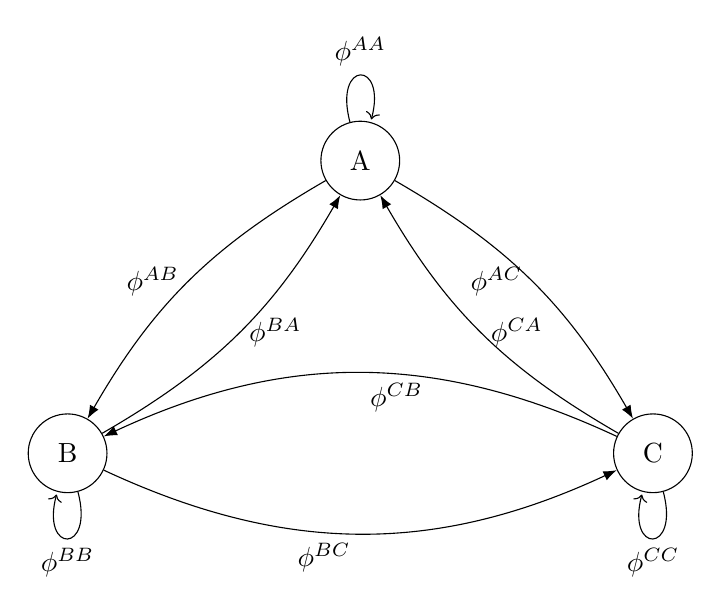
\begin{tikzpicture}[
    node distance=3cm and 3cm,
    mynode/.style={circle, draw, minimum size=1cm},
    arrow/.style={-Latex}
]

% Nodes
\node[mynode] (A) {A};
\node[mynode, below left=of A] (B) {B};
\node[mynode, below right=of A] (C) {C};

% Loops
\draw[arrow] (A) edge[loop above] node{$\phi^{AA}$} (A);
\draw[arrow] (B) edge[loop below] node{$\phi^{BB}$} (B);
\draw[arrow] (C) edge[loop below] node{$\phi^{CC}$} (C);

% Arrows between nodes with less curvature and separate B-C and C-B arrows
\draw[arrow] (A) to[bend right=15] node[left] {$\phi^{AB}$} (B);
\draw[arrow] (B) to[bend right=15] node[right] {$\phi^{BA}$} (A);
\draw[arrow] (A) to[bend left=15] node[left] {$\phi^{AC}$} (C);
\draw[arrow] (C) to[bend left=15] node[right] {$\phi^{CA}$} (A);
\draw[arrow] (B) to[bend right=25] node[below left] {$\phi^{BC}$} (C);
\draw[arrow] (C) to[bend right=25] node[below right] {$\phi^{CB}$} (B);

\end{tikzpicture}
\caption{Schematic representing typical multi-state model. Here, there are 3 states (A, B, and C), with the arrows indicating directional movement between states over a given time interval. The probability of moving, conditional on survival, between state \( i \) and \( j \) is determined by parameter \( \phi_{ij} \).\cite{mark_website}}
\label{fig:multi-state-model}
\end{figure}


\begin{figure}
    \centering
    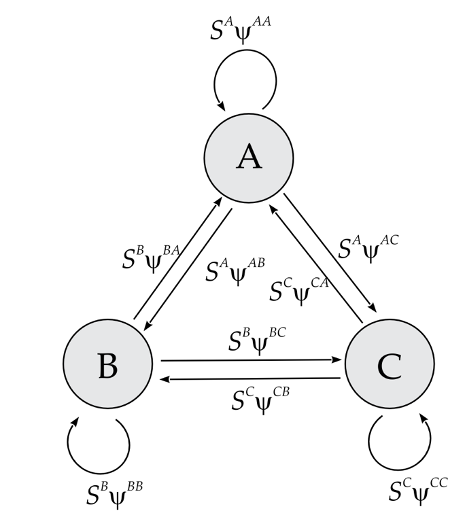
\includegraphics[width=0.5\textwidth]{Picture1} 
    \caption{Re-parameterization of Fig.\ref{fig:multi-state-model}, where $\phi_{ij}$ is partitioned as the product of survival ($S$) and movement ($\psi$).\cite{mark_website}}
    \label{fig:reparameterization}
\end{figure}



\section{Multievent Models: Accounting for Uncertain States}

The evolution of capture–recapture models has progressed from addressing encounter probabilities to encompassing animal movement and state transitions. However, conventional models fall short in accounting for uncertainty in state assignments. This section explores multievent models as an extension of multistate capture–recapture models, incorporating the crucial element of uncertainty in state determination.

Capture–recapture models initially tackled encounter probabilities in free-ranging animal populations. Modern applications extend beyond mere encounter dynamics, capturing the movement of animals across various locations and examining transitions between distinct states. Yet, existing models often overlook uncertainties associated with state assignments.

Multievent models, belonging to the family of hidden Markov models, offer a solution by integrating uncertainty into the assessment of state. These models introduce the concept of events recorded at each sampling occasion, providing a more nuanced perspective than traditional state-based approaches.

The fundamental assumption of the time-dependent multievent model posits that individuals move independently through a defined set of states over multiple sampling occasions. Explicitly, states such as "breeder," "nonbreeder," and "dead" are considered, and events like "sitting on an egg," "standing in the colony," "feeding in a nearby field," and "not observed" are recorded.

\subsubsection*{Model Parameters}

The parameters governing the multievent model include:

\begin{itemize}
    \item $\phi_{ij,t}$: the probability of being in state $e_i$ at time $t + 1$ if being in state $e_i$ at time $t$.
    \item $\pi_{i,t}$: the probability of being in state $e_i$ when first encountered at time $t$.
    \item $b_{uj,t}$: the probability of event $v_u$ for an animal in state $e_j$ at time $t$.
    \item $b_{uj,t}^0$: the probability of event $v_u$ for an animal in state $e_j$ at time $t$, which is then encountered, i.e., $P(v_u | e_j \text{ and “encountered”})$.
\end{itemize}


\subsubsection*{Applications to Breeding States}

Transitions between breeder (B) and nonbreeder (NB) states form a focal point of interest. Three states ($E = \{B, NB, \dag\}$) and three events ($\Omega = \{\text{seen breeding (code 1)}, \text{status unknown (code 2)}, \text{not seen (code 0)}\}$) illustrate the model's versatility.\cite{pradel2005multievent}

\subsubsection*{Model Matrices}

Matrix representations, such as $\Phi_t$ and $\beta_t$, elucidate the probabilities associated with transitioning between states and events. Constraints, such as $b_{12} = 0$, ensure logical interpretations, e.g., a nonbreeder cannot be observed sitting on an egg.

The parameters of the model are, with obvious notations:

\[
\Phi_t = 
\begin{pmatrix}
\phi_{B,B} & \phi_{B,NB} & 1 - \phi_{B,B} - \phi_{B,NB} \\
\phi_{NB,B} & \phi_{NB,NB} & 1 - \phi_{NB,B} - \phi_{NB,NB} \\
0 & 0 & 1 
\end{pmatrix}_t,
\]

\[
B_t = 
\begin{pmatrix}
p_{1|B} & 0 & 0 \\
p_{2|B} & p_{NB} & 0 \\
1 - p_{1|B} - p_{2|B} & 1 - p_{NB} & 1 
\end{pmatrix}_t,
\]

\[
\pi_t = (\pi_1, \pi_2, 0)_t.
\]


\phi_{t} = \begin{pmatrix}
\phi_{CC} & \phi_{CD} & 0 & 0 & 1 - \phi_{CC} - \phi_{CD} & 0 \\
0 & \phi_{DC} & \phi_{DD} & 0 & 1 - \phi_{DC} - \phi_{DD} & 0 \\
\phi_{CC} & \phi_{CD} & 0 & 0 & 1 - \phi_{CC} - \phi_{CD} & 0 \\
0 & 0 & \phi_{DC} & \phi_{DD} & 0 & 1 - \phi_{DC} - \phi_{DD} \\
0 & 0 & 0 & 0 & 0 & 1 \\
0 & 0 & 0 & 0 & 0 & 1
\end{pmatrix}_t,


The formulation allows for calculating the probability that an encountered breeder is engaged in breeding activity ($\beta$). This approach facilitates a nuanced understanding of encounter dynamics, contributing to a more refined interpretation of observed behaviors.



\section{Conclusion}
This study has provided a comprehensive analysis of the Ancient Murrelet (\textit{Synthliboramphus antiquus}), contributing significantly to our understanding of its life cycle, behavior, and survival challenges. Through detailed examination of taxonomy, physical characteristics, global distribution, and foraging behavior, we have gained insights into the unique adaptations and ecological role of this species.

The application of multi-state, multi-event ,and capture–recapture models has been pivotal in assessing the survival dynamics of the Ancient Murrelet, particularly in relation to the cost of reproduction. The analysis of encounter histories and the interplay between survival and movement probabilities have revealed complex patterns in the life cycle of these birds. Our findings indicate that the survival of Ancient Murrelets is intricately linked to their breeding behavior, habitat conditions, and the presence of introduced predators.

This paper lays the groundwork for a brief exploration of multi-state models, setting the stage for specific applications and methodological intricacies within avian ecology.
Multievent models represent a powerful tool in ecological studies, especially when uncertainties in state assignments significantly impact the interpretation of capture–recapture data. The incorporation of hidden Markov principles provides a robust framework for addressing complex scenarios, contributing to a more comprehensive understanding of animal behavior and population dynamics.

Moving forward, the next phase of this research involves the practical application of these sophisticated models to the empirical data of Ancient Murrelets. By leveraging these advanced methodologies, we aim to unravel the complexities inherent in the breeding, survival, and movement patterns of this avian species. The integration of uncertainty considerations, as demonstrated in multievent models, holds particular promise in providing a more accurate and realistic depiction of the Ancient Murrelet's life history.

\bibliographystyle{plain} % We choose the "plain" reference style
\bibliography{Resources1} % Entries are in the refs.bib file
	


\end{document}



